\documentclass[11pt,a4paper]{article}
\usepackage[utf8]{inputenc}
\usepackage[T1]{fontenc}
\usepackage{tgpagella}
\usepackage[spanish]{babel}
\usepackage{geometry}
\usepackage{booktabs}
\usepackage{xcolor}
\usepackage{titlesec}
\usepackage{fancyhdr}
\usepackage[parfill]{parskip}
\usepackage[expansion=false]{microtype}
\usepackage{hyperref}
\usepackage{setspace}
\usepackage{needspace}
\usepackage{graphicx}
\widowpenalty=10000
\clubpenalty=10000
\displaywidowpenalty=10000

\geometry{top=3.0cm,bottom=3.0cm,left=3.5cm,right=3.5cm}
\setlength{\parskip}{0.65em}
\setlength{\parindent}{0em}

\definecolor{azulai}{RGB}{30,80,140}
\definecolor{doradoai}{RGB}{140,90,0}
\definecolor{grisai}{RGB}{70,70,70}

\titleformat{\section}{\Large\bfseries\color{azulai}}{}{0em}{}[{\color{azulai}\titlerule[0.5pt]}]
\titlespacing*{\section}{0pt}{1.8em}{0.8em}
\titleformat{\subsection}{\large\bfseries\color{doradoai}}{}{0em}{}
\titlespacing*{\subsection}{0pt}{1.4em}{0.5em}
\titleformat{\subsubsection}{\normalsize\bfseries\color{grisai}}{}{0em}{}
\titlespacing*{\subsubsection}{0pt}{1.0em}{0.3em}

\pagestyle{fancy}\fancyhf{}
\rhead{\textcolor{grisai}{\small Izas — Arquitectura Interna}}
\lhead{\textcolor{grisai}{\small Júpiter · Saturno}}
\cfoot{\textcolor{grisai}{\small\thepage}}
\renewcommand{\headrulewidth}{0.3pt}

\hypersetup{colorlinks=true,linkcolor=azulai,urlcolor=azulai}
\setstretch{1.45}
\tolerance=1500
\emergencystretch=4em

\begin{document}

% ── Portada ──────────────────────────────────────────────────────────────────

\begin{titlepage}
\centering

\vspace*{2cm}

{\Huge\bfseries\color{azulai} Júpiter · Saturno}\\[0.4cm]

{\large\color{grisai} Arquitectura Interna}\\[0.25cm]

{\small\itshape\color{grisai}
Crecimiento, estructura y organización interna
}\\[1.8cm]

{\huge\color{doradoai} Izas}\\[1.2cm]

{\Large 16/04/1979 \quad 04:20}\\[0.25cm]

{\Large Pamplona, España}\\[0.25cm]

{\normalsize
Lat: 42.8157° \quad
Lon: -1.6522° \quad
UTC+02:00
}\\[0.4cm]

{\normalsize
Ascendente: Acuario 6°20'
\quad
MC: Escorpio 29°12'
}\\[1.6cm]

\begin{tabular}{ll}
\textbf{Júpiter:} & Cáncer — Casa 6 29°42' \\
\textbf{Saturno:} & Virgo — Casa 7 7°33' (Retrógrado) \\
\end{tabular}

\vfill

{\small\color{grisai}
Generado el 19/05/2026
}

\end{titlepage}

	ableofcontents
space{0.8cm}

% ── Datos de referencia ──────────────────────────────────────────────────────

\section{Datos de referencia}

\begin{center}
\begin{tabular}{llll}
\toprule
\textbf{Punto} & \textbf{Signo} & \textbf{Casa} & \textbf{Posición} \\
\midrule

Júpiter &
Cáncer &
Casa 6 &
29°42' \\

Saturno (Retrógrado) &
Virgo &
Casa 7 &
7°33' \\

Sol &
Aries &
Casa 2 &
25°31' \\

Luna &
Sagitario &
Casa 10 &
8°24' \\

Mercurio &
Piscis &
Casa 2 &
28°57' \\

Venus &
Piscis &
Casa 1 &
21°30' \\

Marte &
Aries &
Casa 2 &
7°01' \\

Urano &
Escorpio &
Casa 9 &
19°58' \\

Ascendente &
Acuario &
--- &
6°20' \\

Medio Cielo &
Escorpio &
--- &
29°12' \\

\bottomrule
\end{tabular}
\end{center}

\vspace{0.8cm}

\subsection*{Aspectos entre funciones}

\begin{center}
\begin{tabular}{lllll}
  \toprule
  \textbf{Planeta 1} & \textbf{Asp.} & \textbf{Planeta 2} & \textbf{Tipo} & \textbf{Orbe} \\
  \midrule
  Júpiter & tri & Mercurio & Trígono & 0.8° \\
  Saturno & cua & Luna & Cuadratura & 0.8° \\
  Saturno & tri & Quirón & Trígono & 1.7° \\
  Júpiter & cua & Sol & Cuadratura & 4.2° \\
  Júpiter & tri & Marte & Trígono & 7.3° \\
  \bottomrule
\end{tabular}
\end{center}

\vspace{1cm}

\begin{center}
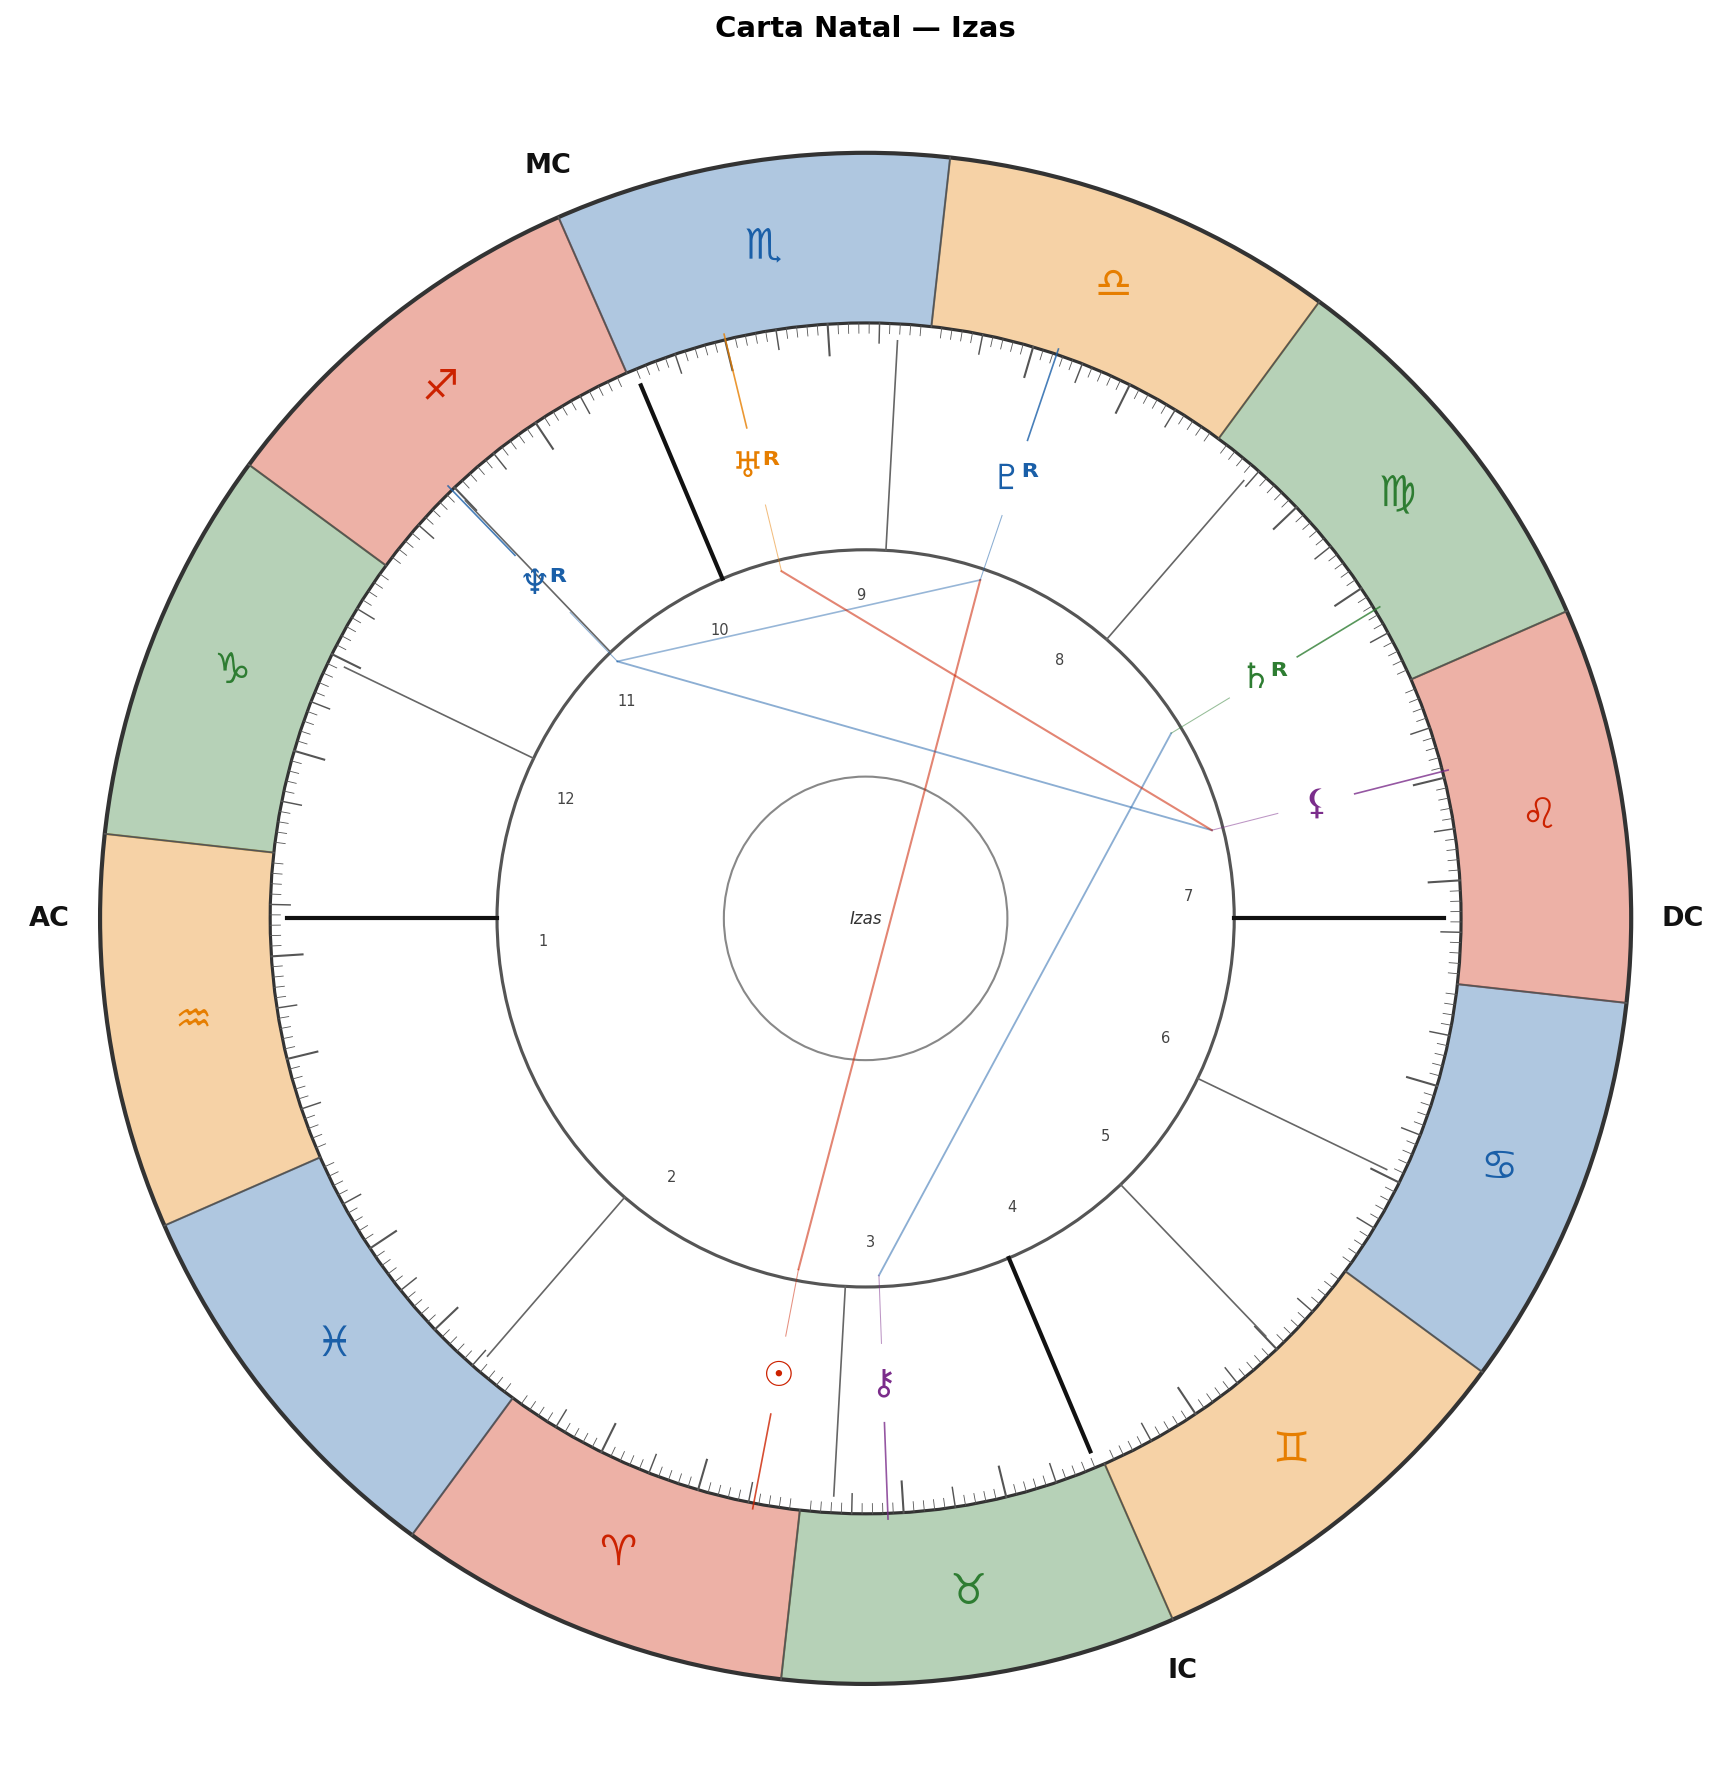
\includegraphics[width=0.72\textwidth]{Izas_rueda.png}
\end{center}

\vspace{0.8cm}
\Needspace{5\baselineskip}


% ── Interpretación ───────────────────────────────────────────────────────────

\section{Interpretación — Arquitectura Interna}

\begin{center}
{\small\itshape
No se trata de definir quién eres.\\
Se trata de observar cómo tiendes a crecer, estructurarte\\
y sostener tu relación con el mundo.
}
\end{center}

\vspace{0.8cm}
\Needspace{5\baselineskip}

% ── 1. Estructura general ────────────────────────────────────────────────────

\subsection{1. Estructura general}

Júpiter está en Cáncer, Casa 6: muestra cómo tiendes a crecer, abrir posibilidades y ampliar tu relación con el mundo.
Saturno está en Virgo, Casa 7: muestra cómo tiendes a estructurarte, sostener límites y construir estabilidad.

Expansión (Cáncer, Agua) y estructura (Virgo, Tierra) operan en elementos compatibles. Esto puede facilitar que crecimiento y sostén colaboren con relativa naturalidad, aunque cada uno tenga un ritmo distinto.

Aspectos relevantes: Júpiter–Sol en cuadratura (orbe 4.19°), Júpiter–Mercurio en trígono (orbe 0.75°), Júpiter–Marte en trígono (orbe 7.32°), Saturno–Luna en cuadratura (orbe 0.85°).

\vspace{0.8cm}
\Needspace{5\baselineskip}

% ── 2. Júpiter ───────────────────────────────────────────────────────────────

\subsection{2. Júpiter — Expansión y crecimiento}

\subsubsection*{
Júpiter en Cáncer
— Casa 6
}

Tiendes a crecer a través del cuidado, la pertenencia y la construcción de vínculos significativos. La expansión aparece cuando sientes conexión emocional con lo que haces, construyes o sostienes. Necesitas seguridad afectiva para abrirte al crecimiento.

En situaciones de desbordamiento: puedes asumir más responsabilidad emocional de la que realmente puedes sostener. La necesidad de cuidar puede hacer que te olvides de tus propios límites. En momentos de estancamiento: si no sientes suficiente seguridad o protección, tiendes a cerrarte antes que a expandirte. La necesidad de resguardo puede frenar movimientos importantes.

Tiendes a crecer a través del trabajo cotidiano, el aprendizaje práctico y la mejora constante. La expansión aparece cuando puedes desarrollar habilidades útiles y organizar tu vida de forma más eficiente y coherente. Necesitas sentir que lo que haces tiene función y aporta algo concreto.

Júpiter cuadratura Sol: la necesidad de crecer y la dirección que intentas sostener generan tensión. Puedes querer expandirte más allá de lo que realmente puedes integrar o sentir que la dirección actual resulta demasiado estrecha para lo que necesitas desarrollar.

La dificultad suele aparecer al medir límites, ritmos y capacidad real de sostén.

\vspace{0.8cm}
\Needspace{5\baselineskip}

% ── 3. Saturno ───────────────────────────────────────────────────────────────

\subsection{3. Saturno — Estructura y sostén}

\subsubsection*{
Saturno en Virgo
— Casa 7 (Retrógrado)
}

Tiendes a estructurarte a través del orden, la precisión y la mejora constante. Necesitas procedimientos claros, coherencia funcional y sensación de utilidad real para sostenerte. La estructura aparece refinando continuamente lo que haces.

El límite aparece en el desgaste de intentar mantener estándares demasiado altos de forma permanente. No todo puede estar completamente bajo control.

Cuando la estructura deja de sostenerse: aparece exceso de análisis, ansiedad funcional o necesidad de corregir continuamente. La organización consume más energía de la que realmente aporta.

Tiendes a estructurarte a través de los compromisos y las relaciones de largo plazo. Necesitas vínculos relativamente sólidos, claros y sostenibles para sentir coherencia. Las relaciones suelen vivirse con seriedad y sentido de responsabilidad.

El límite aparece en los vínculos que no pueden sostener reciprocidad, compromiso o estabilidad suficiente. Las relaciones demasiado ambiguas o inconsistentes generan mucho desgaste.

Saturno está retrógrado. La construcción de estructura suele desarrollarse de forma más interna y menos visible desde fuera al principio. Puedes necesitar tiempo antes de mostrar externamente algo que por dentro todavía estás consolidando.

Saturno cuadratura Luna: estructura y regulación emocional están en tensión. Puedes sentir que necesitas controlarte para sostener estabilidad o que lo emocional interrumpe la estructura que intentas construir.

La dificultad suele estar en permitir emoción sin perder sostén y sostén sin bloquear completamente la emoción.

\vspace{0.8cm}
\Needspace{5\baselineskip}

% ── 4. Integración ───────────────────────────────────────────────────────────

\subsection{4. Integración — Crecimiento y estructura}

Júpiter en Cáncer y Saturno en Virgo no forman aspecto directo y operan en elementos compatibles. La integración entre crecimiento y estructura tiene menor fricción de base. Precisamente por eso, conviene no asumir que se regulan solas: puedes entrar en sobreextensión o en rigidez progresiva sin detectarlo hasta que el coste ya es alto.

Cuando Júpiter domina: puedes absorber demasiado emocionalmente hasta perder la referencia de lo propio. La estructura de Saturno en Virgo no compensa con suficiente rapidez y lo que ganas en amplitud empieza a perder forma.

Cuando Saturno domina: puedes acumular tanta estructura que la forma termina impidiendo el movimiento. La expansión de Júpiter en Cáncer no encuentra espacio para activarse y puedes mantener lo que ya existe sin crecer hacia lo que sería posible.

Bajo presión suele aparecer una secuencia bastante reconocible. Primero, Saturno en Virgo empieza a ceder: pierdes estructura antes de haber construido una nueva base que la sustituya. Después, Júpiter en Cáncer ocupa ese espacio: absorbes demasiado de lo que ocurre alrededor sin poder procesarlo o diferenciarlo bien. Desde ahí puedes intentar recuperar estabilidad rápidamente, pero lo que construyes en ese estado suele ser más rígido, reactivo o agotador de sostener. Si el patrón no se reconoce a tiempo, el ciclo tiende a repetirse.

\vspace{0.8cm}
\Needspace{5\baselineskip}

% ── 5. Orientación práctica ──────────────────────────────────────────────────

\subsection{5. Orientación práctica}

\subsubsection*{Desde dónde empezar}

El punto de entrada más accesible suele estar en la estructura (Virgo, Casa 7). De las dos funciones, esta requiere menos resistencia para activarse. La forma más natural de empezar es llevar lo que ocurre a algo concreto, verificable y práctico. Cuando todo parece bloqueado, comenzar por aquí suele facilitar que la otra función también pueda ponerse en marcha.

\subsubsection*{Qué sostener}

Lo más importante de sostener aparece en Saturno (Virgo, Casa 7). Bajo presión puedes abrir posibilidades o reaccionar antes de mantener forma estable. Conviene cuidar especialmente mantener una estructura concreta aunque sea pequeña o sencilla. Muchas veces la primera señal de desgaste aparece cuando sigues haciendo cosas, pero ya no existe suficiente estructura para sostenerlas bien.

\subsubsection*{Qué evitar}

Conviene evitar asumir que la compatibilidad entre crecimiento y estructura garantiza integración automática. Cuando no existe fricción visible, ciertos desequilibrios pueden acumularse durante bastante tiempo antes de hacerse evidentes.

\subsubsection*{Si no se integra}

Cuando crecimiento y estructura dejan de colaborar, puede aparecer expansión sin suficiente sostén o estabilidad sin movimiento real. En ambos casos se pierde parte de lo que realmente podría desarrollarse si ambas funciones trabajaran en la misma dirección.

\subsubsection*{Señal temprana}

La primera señal suele aparecer en Saturno (Virgo): la acumulación empieza a superar la capacidad real de gestión. Cuando eso ocurre, Júpiter (Cáncer) tiende a ocupar rápidamente el espacio disponible y la expansión puede acelerarse más de lo que realmente puedes sostener. Detectar la señal temprano suele evitar entrar en ciclos más agotadores.

\vfill

\begin{center}
{\small\itshape\color{grisai}
La astrología se utiliza aquí como herramienta simbólica de observación\\
y no como una definición cerrada de la persona.
}
\end{center}

\end{document}
